\documentclass{article}
\usepackage{minted}
\usepackage[spanish]{babel}
\usepackage{hyperref}
\usepackage{graphicx}
\graphicspath{ {./images/} }

%%%%%%%%%%%%%%%%%%%%%%%%%%%%%%%%%%%%%%%%%%%%%%%%%%%%%%
% COMIENZA EL DOCUMENTO
%%%%%%%%%%%%%%%%%%%%%%%%%%%%%%%%%%%%%%%%%%%%%%%%%%%%%%

\begin{document}

\tableofcontents

\section{Túneles 6in4}
Dado el siguiente escenario:

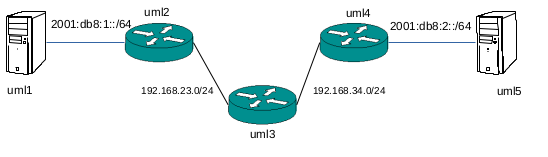
\includegraphics[width=\textwidth]{tuneles6in4}

\begin{minted}{bash}
  # net.conf
  defsw br12 uml1.0 uml2.0
  defsw br23 uml2.1 uml3.0
  defsw br34 uml3.1 uml4.0
  defsw br23 uml4.1 uml5.0
\end{minted}

\begin{minted}{lexer.py:IOSLexer -x}
  ! UML1 y UML5
  configure terminal
  int eth0
  no shutdown
  end
  write
\end{minted}

\begin{minted}{lexer.py:IOSLexer -x}
 ! UML2
 configure terminal
 int eth0
 ipv6 address 2001:db8:1::1/64
 ipv6 nd prefix 2001:db8:1::/64 ! Para que anuncie su prefijo a UML1
 no ipv6 nd suppress-ra
 quit
 int eth1
 ip address 192.168.23.1/24
 quit
 ip route 0.0.0.0/0 192.168.23.2
 ipv6 forwarding
 ip forwarding
 end
 write
\end{minted}

\begin{minted}{lexer.py:IOSLexer -x}
 ! UML3
 configure terminal
 int eth0
 ip address 192.168.23.2/24
 quit
 int eth1
 ip address 192.168.34.2/24
 quit
 ip forwarding
 ip route 192.168.23.0/24 192.168.34.2
 ip route 192.168.34.0/24 192.168.23.2
 end
 write
\end{minted}

\begin{minted}{lexer.py:IOSLexer -x}
 ! UML4
 configure terminal
 int eth0
 ip address 192.168.34.1/24
 quit
 int eth1
 ipv6 address 2001:db8:2::1/64
 ipv6 nd prefix 2001:db8:2::/64 ! Para que anuncie su prefijo a UML5
 no ipv6 nd suppress-ra
 quit
 ip route 0.0.0.0/0 192.168.34.2
 ipv6 forwarding
 ip forwarding
 end
 write
\end{minted}

\begin{minted}{bash}
 # UML2 (bash)
 ip tunnel add tunnel1 mode sit remote 192.168.34.1
 ip link set dev tunnel1 up mtu 1400
 ip route add 2001:db8:2::/64 dev tunnel1
\end{minted}

\begin{minted}{bash}
 # UML4 (bash)
 ip tunnel add tunnel2 mode sit remote 192.168.23.1
 ip link set dev tunnel2 up mtu 1400
 ip route add 2001:db8:1::/64 dev tunnel2
\end{minted}

\begin{minted}{lexer.py:IOSLexer -x}
 # TEST
 # probar desde vtysh en UML1 y UML2 que se anunció correctamente el prefijo
 show ipv6 route
\end{minted}

\begin{minted}{bash}
 # TEST
 # Desde UML2, probar un ping a UML4 y viceversa
 ping -c 5 192.168.(34|23).1
 # Desde UML1, probar un ping6 a UML5 y viceversa
 ping6 -c 5 2001:db8:(1|2):ff:fe00:5f0
\end{minted}


\section{OSPFv2}

Configurar 5 máquinas virtuales para crear el siguiente AS:

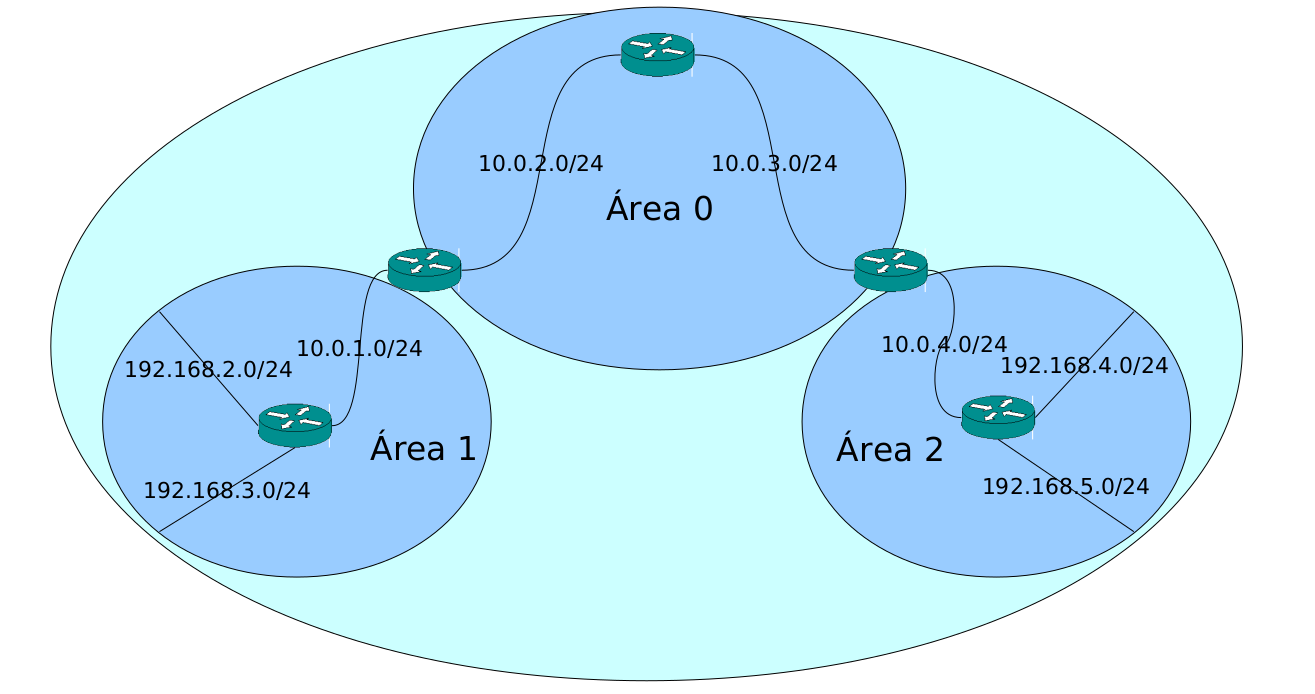
\includegraphics[width=\textwidth]{ospfv2}

\begin{minted}{bash}
  # net.conf
  defsw br12 uml1.0 uml2.0
  defsw net1 uml1.1
  defsw net2 uml1.2
  defsw br23 uml2.1 uml3.0
  defsw br34 uml3.1 uml4.0
  defsw br45 uml4.1 uml5.0
  defsw net3 uml5.1
  defsw net4 uml5.2
\end{minted}

\begin{minted}{bash}
  # En cuanto se inician las UML, editar el fichero /etc/quagga/daemons la línea
  ospfd=no
  # Por
  ospfd=yes
  # A continuación restart del servicio
  systemctl restart quagga
  # Verificar que se ospfd está corriendo
  systemctl status quagga
\end{minted}

\begin{minted}{lexer.py:IOSLexer -x}
 ! UML1 (zebra.conf)
 conf[igure] term[inal]
 int[erface] eth0
 ip address 10.0.1.1/24
 no shutdown
 quit
 int[erface] eth1
 ip address 192.168.3.1/24
 no shutdown
 quit
 int[erface] eth2
 ip address 192.168.2.1/24
 no shutdown
 quit
 ip forwarding
 exit
 write
\end{minted}
\begin{minted}{lexer.py:IOSLexer -x}
 ! UML2 (zebra.conf)
 conf[igure] term[inal]
 int[erface] eth0
 ip address 10.0.1.2/24
 no shutdown
 quit
 int[erface] eth1
 ip address 10.0.2.2/24
 no shutdown
 quit
 ip forwarding
 exit
 write
\end{minted}

\begin{minted}{lexer.py:IOSLexer -x}
 ! UML3 (zebra.conf)
 conf[igure] term[inal]
 int[erface] eth0
 ip address 10.0.2.1/24
 no shutdown
 quit
 int[erface] eth1
 ip address 10.0.3.1/24
 no shutdown
 quit
 ip forwarding
 exit
 write
\end{minted}

\begin{minted}{lexer.py:IOSLexer -x}
 ! UML4 (zebra.conf)
 conf[igure] term[inal]
 int[erface] eth0
 ip address 10.0.3.2/24
 no shutdown
 quit
 int[erface] eth1
 ip address 10.0.4.2/24
 no shutdown
 quit
 ip forwarding
 exit
 write
\end{minted}

\begin{minted}{lexer.py:IOSLexer -x}
 ! UML5 (zebra.conf)
 conf[igure] term[inal]
 int[erface] eth0
 ip address 10.0.4.1/24
 no shutdown
 quit
 int[erface] eth1
 ip address 192.168.4.1/24
 no shutdown
 quit
 int[erface] eth2
 ip address 192.168.5.1/24
 no shutdown
 quit
 ip forwarding
 exit
 write
\end{minted}

\begin{minted}{lexer.py:IOSLexer -x}
 ! UML1 ospf.conf
 conf[igure] term[inal]
 router ospf
 ospf router-id 0.0.0.1
 network 10.0.1.0/24 area 1
 network 192.168.2.0/24 area 1
 network 192.168.3.0/24 area 1
 area 1 stub
 passive-interface eth1 ! Las redes de usuario irán siempre como passive-interface
 passive-interface eth2
 end
 write
\end{minted}

\begin{minted}{lexer.py:IOSLexer -x}
 ! UML2 ospf.conf
 conf[igure] term[inal]
 router ospf
 ospf router-id 0.0.0.2
 network 10.0.1.0/24 area 1
 network 10.0.2.0/24 area 0
 ! No advierte de este area en otras areas por ser ABR
 area 1 range 10.0.0.0/8 not-advertise
 end
 write
\end{minted}

\begin{minted}{lexer.py:IOSLexer -x}
 ! UML3 ospf.conf
 conf[igure] term[inal]
 router ospf
 ospf router-id 0.0.0.3
 network 10.0.2.0/24 area 0
 network 10.0.3.0/24 area 0

\end{minted}

\begin{minted}{lexer.py:IOSLexer -x}
 ! UML4 ospf.conf
 conf[igure] term[inal]
 router ospf
 ospf router-id 0.0.0.4
 network 10.0.3.0/24 area 0
 network 10.0.4.0/24 area 2
 ! No advierte de este area en otras areas por ser ABR
 area 2 range 10.0.0.0/8 not-advertise
 end
 write
\end{minted}

\begin{minted}{lexer.py:IOSLexer -x}
 ! UML5 ospf.conf
 conf[igure] term[inal]
 router ospf
 ospf router-id 0.0.0.5
 network 10.0.4.0/24 area 2
 network 192.168.4.0/24 area 2
 network 192.168.5.0/24 area 2
 area 2 stub
 passive-interface eth1 ! Las redes de usuario irán siempre como passive-interface
 passive-interface eth2
 end
 write
\end{minted}

Comprobar las tablas de ospf con el comando

\begin{minted}{lexer.py:IOSLexer -x}
 show ip ospf database
\end{minted}

\newpage
\section{OSPFv3}
Configurar 5 máquinas virtuales para crear el siguiente AS:

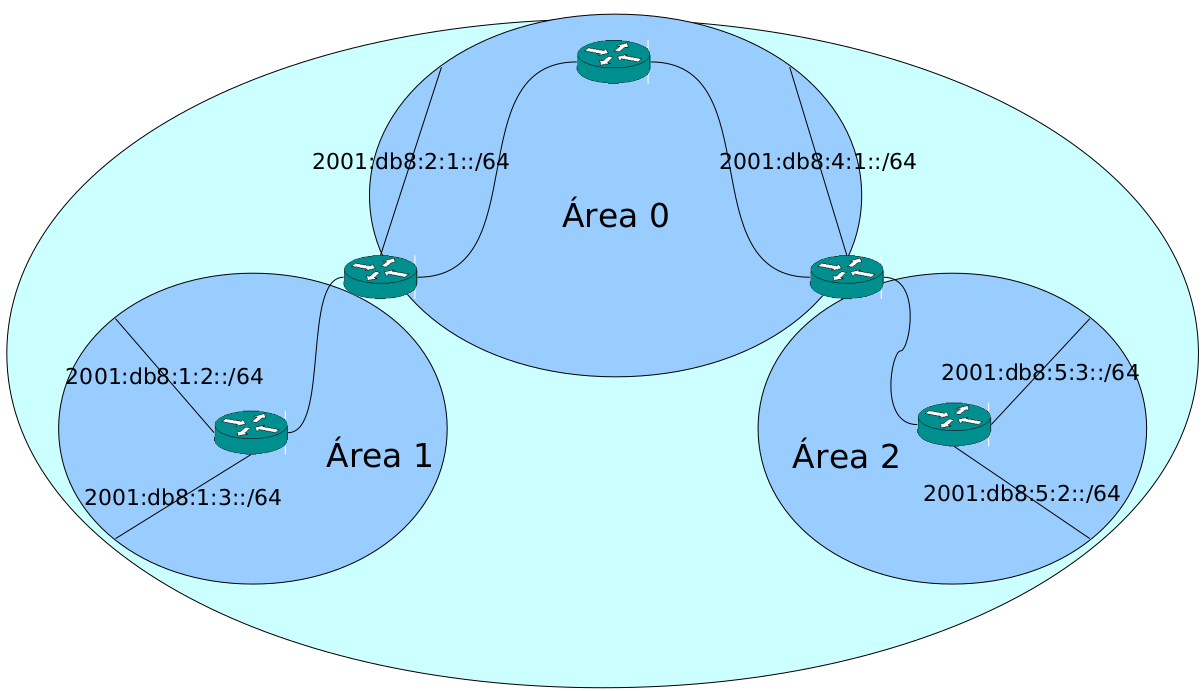
\includegraphics[width=\textwidth]{ospfv3}

\begin{minted}{bash}
 # net.conf
 defsw br12 uml1.0 uml2.0
 defsw net1 uml1.1
 defsw net2 uml1.2
 defsw br23 uml2.2 uml3.0
 defsw net3 uml2.1
 defsw br34 uml3.1 uml4.0
 defsw net4 uml4.2
 defsw br45 uml4.1 uml5.0
 defsw net5 uml5.1
 defsw net6 uml5.2
\end{minted}

\begin{minted}{bash}
  # En cuanto se inician las UML, editar el fichero /etc/quagga/daemons la línea
  ospf6d=no
  # Por
  ospf6d=yes
  # A continuación restart del servicio
  systemctl restart quagga
  # Verificar que se ospfd está corriendo
  systemctl status quagga
\end{minted}

\begin{minted}{lexer.py:IOSLexer -x}
 ! UML1 zebra.conf
 conf[igure] term[inal]
 int[erface] eth0
 no shutdown
 quit
 int[erface] eth1
 ipv6 address 2001:db8:1:3::1/64
 no shutdown
 quit
 int[erface] eth2
 ipv6 address 2001:db8:1:2::1/64
 no shutdown
 quit
 ipv6 forwarding
 exit
 write
\end{minted}

\begin{minted}{lexer.py:IOSLexer -x}
 ! UML2 zebra.conf
 conf[igure] term[inal]
 int[erface] eth0
 no shutdown
 quit
 int[erface] eth1
 ipv6 address 2001:db8:2:1::1/64
 no shutdown
 quit
 int[erface] eth2
 no shutdown
 quit
 ipv6 f[orwarding]
 exit
 write
\end{minted}

\begin{minted}{lexer.py:IOSLexer -x}
 ! UML3 zebra.conf
 conf[igure] term[inal]
 int[erface] eth0
 no shutdown
 quit
 int[erface] eth1
 no shutdown
 quit
 ipv6 f[orwarding]
 exit
 write
\end{minted}

\begin{minted}{lexer.py:IOSLexer -x}
 ! UML4 zebra.conf
 conf[igure] term[inal]
 int[erface] eth0
 no shutdown
 quit
 int[erface] eth1
 no shutdown
 quit
 int[erface] eth2
 ipv6 address 2001:db8:4:1::1/64
 no shutdown
 quit
 ipv6 f[orwarding]
 exit
 write
\end{minted}

\begin{minted}{lexer.py:IOSLexer -x}
 ! UML5 zebra.conf
 conf[igure] term[inal]
 int[erface] eth0
 no shutdown
 quit
 int[erface] eth1
 ipv6 address 2001:db8:5:3::1/64
 no shutdown
 quit
 int[erface] eth2
 ipv6 address 2001:db8:5:2::1/64
 no shutdown
 quit
 ipv6 forwarding
 exit
 write
\end{minted}

\begin{minted}{lexer.py:IOSLexer -x}
 ! UML1 ospf6d.conf
 conf[igure] term[inal]
 router ospf6
 router-id 0.0.0.1
 interface eth0 area 0.0.0.1
 interface eth1 area 0.0.0.1
 interface eth2 area 0.0.0.1
 end
 write
\end{minted}

\begin{minted}{lexer.py:IOSLexer -x}
 ! UML2 ospf6d.conf
 conf[igure] term[inal]
 router ospf6
 router-id 0.0.0.2
 interface eth0 area 0.0.0.1
 interface eth1 area 0.0.0.0
 interface eth2 area 0.0.0.0
 end
 write
\end{minted}

\begin{minted}{lexer.py:IOSLexer -x}
 ! UML3 ospf6d.conf
 conf[igure] term[inal]
 router ospf6
 router-id 0.0.0.3
 interface eth0 area 0.0.0.0
 interface eth1 area 0.0.0.0
 end
 write
\end{minted}

\begin{minted}{lexer.py:IOSLexer -x}
 ! UML4 ospf6d.conf
 conf[igure] term[inal]
 router ospf6
 router-id 0.0.0.4
 interface eth0 area 0.0.0.0
 interface eth1 area 0.0.0.2
 interface eth2 area 0.0.0.0
 end
 write
\end{minted}

\begin{minted}{lexer.py:IOSLexer -x}
 ! UML5 ospf6d.conf
 conf[igure] term[inal]
 router ospf6
 router-id 0.0.0.5
 interface eth0 area 0.0.0.2
 interface eth1 area 0.0.0.2
 interface eth2 area 0.0.0.2
\end{minted}

\section{BGP, OSPFv2 y OSPFv3}
  Configurar como principales los enlaces marcados:
  \begin{figure}[h]
    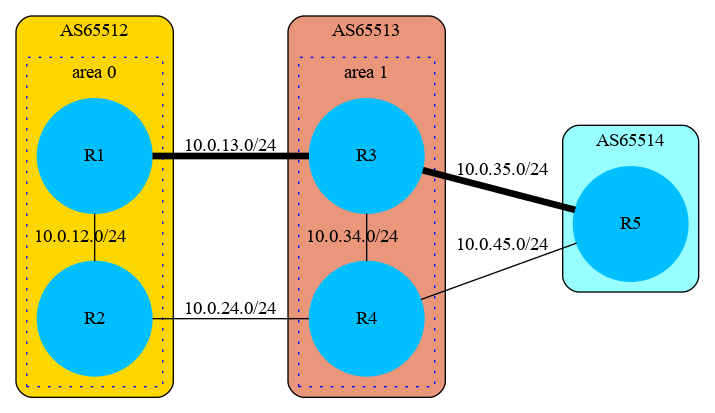
\includegraphics[width=12cm]{bgp_next_hop.png}
  \end{figure}
  
  Detalles a tener en cuenta:
  
  \begin{itemize}
    \item Las interfaces entre los nodos R1 - R3 y R2 - R4 han de ser pasivas
    \item La comunicación entre routeres del mismo AS es mediante iBGP/OSPF
    \item La comunicación entre los AS es mediante eBGP
    \item En el AS 65514 la comunicación con el router R5 es exclusivamente BGP
    \item Anuncios BGP explícitos:
    \begin{itemize}
      \item AS 65512: 172.12.0.0/16
      \item AS 65513: 172.13.0.0/16
      \item AS 65514: 172.14.0.0/16
    \end{itemize}
  \end{itemize}

  \begin{minted}{bash}
    # net.conf
    defsw br12 uml1.0 uml2.0
    defsw br13 uml1.1 uml3.0
    defsw br24 uml2.1 uml4.0
    defsw br34 uml3.1 uml4.1
    defsw br45 uml4.2 uml5.0
    defsw br35 uml3.2 uml5.1
  \end{minted}
  
  \begin{minted}{bash}
  # En cuanto se inician las UML1-4, editar el fichero /etc/quagga/daemons la línea
  bgpd=no
  ospfd=no
  # Por
  bgpd=yes
  ospfd=yes
  # Para UML5, solo cambiar el demonio bgpd=no por bgpd=yes
  # A continuación restart del servicio para todas las UML
  systemctl restart quagga
  # Verificar que se ospfd está corriendo
  systemctl status quagga
\end{minted}
  
  \begin{minted}{lexer.py:IOSLexer -x}
    ! UML1 (zebra.conf)
    conf[igure] term[inal]
    int[erface] eth0
    ip address 10.0.12.1/24
    no shutdown
    quit
    int[erface] eth1
    ip address 10.0.13.1/24
    no shutdown
    quit
    ip forwarding
    exit
    write
  \end{minted}
  
  \begin{minted}{lexer.py:IOSLexer -x}
    ! UML2 (zebra.conf)
    conf[igure] term[inal]
    int[erface] eth0
    ip address 10.0.12.2/24
    no shutdown
    quit
    int[erface] eth1
    ip address 10.0.24.1/24
    no shutdown
    quit
    ip forwarding
    exit
    write
  \end{minted}

  \begin{minted}{lexer.py:IOSLexer -x}
    ! UML3 (zebra.conf)
    conf[igure] term[inal]
    int[erface] eth0
    ip address 10.0.13.1/24
    no shutdown
    quit
    int[erface] eth1
    ip address 10.0.34.1/24
    no shutdown
    int[erface] eth2
    ip address 10.0.35.1/24
    no shutdown
    quit
    ip forwarding
    exit
    write
  \end{minted}
  
  \begin{minted}{lexer.py:IOSLexer -x}
    ! UML4 (zebra.conf)
    conf[igure] term[inal]
    int[erface] eth0
    ip address 10.0.24.2/24
    no shutdown
    quit
    int[erface] eth1
    ip address 10.0.34.2/24
    no shutdown
    int[erface] eth2
    ip address 10.0.45.1/24
    no shutdown
    quit
    ip forwarding
    exit
    write
  \end{minted}
  
  \begin{minted}{lexer.py:IOSLexer -x}
    ! UML5 (zebra.conf)
    conf[igure] term[inal]
    int[erface] eth0
    ip address 10.0.45.2/24
    no shutdown
    quit
    int[erface] eth1
    ip address 10.0.35.2/24
    no shutdown
    quit
    ip forwarding
    exit
    write
  \end{minted}
  
  \begin{minted}{lexer.py:IOSLexer -x}
    ! UML1 (ospf.conf)
    conf[igure] term[inal]
    router ospf
    ospf router-id 0.0.0.1
    network 10.0.12.0/24 area 0
    network 10.0.13.0/24 area 0
    p[assive-interface] eth1 ! El interfaz que comunica con el AS65513
    end
    write
  \end{minted}
  
  \begin{minted}{lexer.py:IOSLexer -x}
    ! UML2 (ospf.conf)
    conf[igure] term[inal]
    router ospf
    ospf router-id 0.0.0.2
    network 10.0.12.0/24 area 0
    network 10.0.24.0/24 area 0
    p[assive-interface] eth1 ! El interfaz que comunica con el AS65513
    end
    write
  \end{minted}

  \begin{minted}{lexer.py:IOSLexer -x}
    ! UML3 (ospf.conf)
    conf[igure] term[inal]
    router ospf
    ospf router-id 0.0.0.3
    network 10.0.13.0/24 area 1
    network 10.0.34.0/24 area 1
    network 10.0.35.0/24 area 1
    p[assive-interface] eth0 ! El interfaz que comunica con el AS65512
    end
    write
  \end{minted}
  
  \begin{minted}{lexer.py:IOSLexer -x}
    ! UML4 (ospf.conf)
    conf[igure] term[inal]
    router ospf
    ospf router-id 0.0.0.4
    network 10.0.24.0/24 area 1
    network 10.0.34.0/24 area 1
    network 10.0.35.0/24 area 1
    p[assive-interface] eth0 ! El interfaz que comunica con el AS65512
    end
    write
  \end{minted}
  
  \begin{minted}{lexer.py:IOSLexer -x}
    ! UML1 (bgp.conf)
    con[figure] t[erminal]
    router bgp 65512
    nei[ghbor] 10.0.13.2 remote-as 65513
    nei[ghbor] 10.0.12.2 remote-as 65512
    network 172.12.0.0/16
    nei[ghbor] 10.0.13.2 route-m[ap] FILTRO in
    route-map FILTRO permit 10
      se[t] l[ocal-preference] 200
    do write
  \end{minted}
  
  \begin{minted}{lexer.py:IOSLexer -x}
    ! UML2 (bgp.conf)
    con[figure] t[erminal]
    router bgp 65512
    nei[ghbor] 10.0.24.2 remote-as 65513
    nei[ghbor] 10.0.12.1 remote-as 65512
    do write
  \end{minted}
  
  \begin{minted}{lexer.py:IOSLexer -x}
    ! UML3 (bgp.conf)
    con[figure] t[erminal]
    router bgp 65513
    nei[ghbor] 10.0.13.1 remote-as 65512
    nei[ghbor] 10.0.35.2 remote-as 65514
    nei[ghbor] 10.0.34.2 remote-as 65513
    network 172.13.0.0/16
    nei[ghbor] 10.0.35.2 route-m[ap] FILTRO in
    route-map FILTRO permit 10
      se[t] l[ocal-preference] 200
    do write
  \end{minted}
  
  \begin{minted}{lexer.py:IOSLexer -x}
    ! UML4 (bgp.conf)
    con[figure] t[erminal]
    router bgp 65513
    nei[ghbor] 10.0.24.1 remote-as 65512
    nei[ghbor] 10.0.45.2 remote-as 65514
    nei[ghbor] 10.0.34.1 remote-as 65513
    do write
  \end{minted}
  
  \begin{minted}{lexer.py:IOSLexer -x}
    ! UML5 (bgp.conf)
    con[figure] t[erminal]
    router bgp 65514
    nei[ghbor] 10.0.35.1 remote-as 65513
    nei[ghbor] 10.0.45.1 remote-as 65513
    network 172.14.0.0/16
    do write
  \end{minted}

  Pruebas:
  \begin{minted}{lexer.py:IOSLexer -x}
    ! En una UML
    clear bgp * ! se borra toda la información BGP de las tablas de todos los routeres
    ! En cada uno de los nodos
    sh[ow] ip bgp
  \end{minted}

  \begin{itemize}
    \item Probar a cambiar el router que anuncia la network para comprobar\
    que las rutas BGP son acordes a las políticas aplicadas
  \end{itemize}
\end{document}


